\documentclass[11pt,a4paper]{article}
\usepackage[utf8]{inputenc}
\usepackage[T1]{fontenc}
\usepackage[spanish]{babel}
\usepackage[colorlinks=true,linkcolor=black,urlcolor=blue,citecolor=black]{hyperref}
\usepackage{float}
\usepackage{graphicx}
\usepackage{geometry}
\usepackage{listings}
\usepackage{xcolor}
\usepackage{booktabs}
\usepackage{verbatim}
\usepackage{caption}

\geometry{left=2.5cm,right=2.5cm,top=2.5cm,bottom=2.5cm}

\title{\textbf{Memoria del Análisis Nextflow}\\ \Large Pipeline de RNA-seq en Nextflow (Dataset GSE52778)}
\author{Máster en Bioinformática}
\date{\today}

\author{Miguel Ángel Vicente Mesonero \\ Gloria Muñoz Martín \\ Javier Luque Serrano}

\begin{document}

\maketitle

\begin{abstract}
\noindent Este documento describe el desarrollo, la ejecución y los resultados de un pipeline bioinformático completo para el análisis de datos de RNA-seq del dataset GSE52778. El pipeline fue construido en Nextflow DSL2, integrando contenedores Docker y ejecutado en el HPC Picasso mediante Singularity. A lo largo del proceso, cada herramienta fue encapsulada como módulo independiente, desarrollada y testeada en ramas separadas de GitHub antes de su integración en el flujo principal. Finalmente, se detallan los problemas técnicos encontrados, especialmente en la integración del análisis exploratorio en R, y las soluciones adoptadas.
\end{abstract}

\tableofcontents
\newpage

% =============================================================================
% 1. INTRODUCCIÓN
% =============================================================================
\section{Introducción y Descripción del Pipeline}
\label{sec:intro}

El presente informe recoge la memoria del análisis del pipeline de RNA-seq desarrollado como parte del Módulo 8 de Bioinformática Aplicada del Máster en Bioinformática de la Universidad Europea de Madrid.

El objetivo era construir un pipeline bioinformático reproducible, portable y escalable que integrase contenedores Docker y Nextflow, aplicado a un análisis real de RNA-seq. El dataset seleccionado fue el \textbf{GSE52778}, que contiene datos de secuenciación de células musculares lisas de la vía aérea humana (HASM) de 4 donantes masculinos sanos. Cada donante fue tratado con dexametasona 1$\mu$M durante 18 horas, generando un diseño pareado de 4 $\times$ 2 = 8 muestras (4 no tratadas y 4 tratadas).

El pipeline está diseñado para ejecutarse desde el control de calidad inicial hasta el análisis exploratorio estadístico, con un único comando. Su estructura sigue las mejores prácticas de Nextflow DSL2, donde cada herramienta está encapsulada como un módulo independiente y la ejecución se orquesta desde el archivo principal \texttt{main.nf}.

% =============================================================================
% 2. DESARROLLO DEL PIPELINE
% =============================================================================
\section{Desarrollo del Pipeline: Metodología de Trabajo}
\label{sec:desarrollo}

\subsection{Estrategia de Desarrollo con GitHub}

Durante el desarrollo del pipeline, se adoptó una metodología de trabajo modular y controlada mediante el sistema de control de versiones Git y la plataforma GitHub. \textbf{Cada módulo del pipeline se escribió y testeó de manera independiente utilizando distintas ramas de GitHub} (e.g., \texttt{feature/fastqc}, \texttt{feature/trimmomatic}, \texttt{feature/star-align}).

Esta estrategia permitió:
\begin{itemize}
    \item Aislar el desarrollo de cada herramienta bioinformática, evitando que los errores en un módulo afectaran a los demás.
    \item Realizar pruebas unitarias de cada proceso de Nextflow (\texttt{process}) de forma independiente, ejecutándolo con datos de prueba.
    \item Facilitar la revisión de código y la integración progresiva mediante \textit{Pull Requests}.
    \item Mantener un historial limpio y rastreable de las decisiones técnicas y los cambios realizados.
\end{itemize}

Una vez validado cada módulo en su rama correspondiente, se procedió a la integración en la rama principal (\texttt{main} o \texttt{master}), conectando todos los procesos en el workflow global de \texttt{main.nf}.

\subsection{Integración en el Workflow Principal}

El workflow principal \texttt{main.nf} orquesta la ejecución de los siguientes procesos en orden:

\begin{enumerate}
    \item \textbf{FastQC}: Control de calidad de las lecturas crudas.
    \item \textbf{Trimmomatic}: Eliminación de adaptadores y lecturas de baja calidad.
    \item \textbf{FastQC (post-trim)}: Control de calidad de las lecturas limpias.
    \item \textbf{STAR\_INDEX}: Generación del índice del genoma humano (GRCh38) de una sola vez.
    \item \textbf{STAR\_ALIGN}: Alineamiento de cada muestra al genoma de referencia (8 ejecuciones en paralelo).
    \item \textbf{SAMtools}: Ordenación, indexado y cálculo de métricas de los archivos BAM.
    \item \textbf{Picard MarkDuplicates}: Marcado de duplicados de PCR sin eliminarlos.
    \item \textbf{featureCounts}: Cuantificación de las lecturas por gen, utilizando todos los BAMs simultáneamente.
    \item \textbf{MultiQC}: Agregación de todos los informes de calidad en un único archivo HTML.
\end{enumerate}

Cada proceso se implementa en un archivo separado dentro de \texttt{scripts/modules/}, cumpliendo con los requisitos del DSL2: \texttt{tag}, \texttt{container} (con etiqueta exacta), \texttt{publishDir}, \texttt{input} y \texttt{output} con \texttt{emit} nombrado.

% =============================================================================
% 3. EJECUCIÓN EN HPC PICASSO
% =============================================================================
\section{Ejecución en el HPC Picasso: Perfil Singularity}
\label{sec:picasso}

\subsection{Configuración del Entorno HPC}

El pipeline completo fue ejecutado en el clúster de alto rendimiento (HPC) Picasso, perteneciente al SCBI-UMA. Este clúster utiliza \textbf{Singularity/Apptainer} en lugar de Docker para la gestión de contenedores, y \textbf{Slurm} como gestor de colas de trabajos.

Para adaptar el pipeline a este entorno, se creó un perfil de ejecución específico denominado \textbf{picasso} dentro del archivo \texttt{nextflow.config}. La configuración mínima incluye:

\begin{verbatim}
profiles {
    docker {
        docker.enabled = true
    }
    picasso {
        singularity.enabled    = true
        singularity.autoMounts = true
        singularity.cacheDir = 
            "${System.getenv('HOME')}/.singularity_cache"
    }
}
\end{verbatim}

Esta configuración permite que Nextflow descargue las imágenes Docker definidas en los procesos, las convierta automáticamente a formato \texttt{.sif} (Singularity Image Format) y las ejecute de forma transparente.

\subsection{Ejecución del Pipeline}

El pipeline se lanzó en Picasso utilizando el perfil \texttt{picasso} con el siguiente comando:

\begin{verbatim}
nextflow run scripts/main.nf -profile picasso
\end{verbatim}

Para reanudar una ejecución interrumpida (aprovechando el sistema de caché de Nextflow), se utilizó:

\begin{verbatim}
nextflow run scripts/main.nf -profile picasso -resume
\end{verbatim}

Se debe destacar que la conversión de las imágenes Docker a Singularity es un proceso lento y que consume una cantidad significativa de espacio en disco. Por ello, se configuró el directorio de caché en \texttt{\$HOME} para evitar problemas de cuota en el sistema de archivos temporal \texttt{\$FSCRATCH}. La caché de Singularity \textbf{no debe eliminarse} entre ejecuciones, ya que es la clave para la reanudación eficiente del pipeline.

\subsection{Consideraciones de Recursos}

En Picasso, el paso de \textbf{STAR\_INDEX} es el más exigente en términos de recursos, requiriendo al menos \textbf{64 GB de RAM} y \textbf{12 CPUs} para la indexación del genoma humano completo (GRCh38). En el perfil de configuración, se asignaron los siguientes recursos:

\begin{itemize}
    \item \textbf{STAR\_INDEX} y \textbf{STAR\_ALIGN}: 12 CPUs, 64 GB RAM.
    \item \textbf{Procesos por defecto}: 2 CPUs, 4 GB RAM.
\end{itemize}

La ejecución local de todo el pipeline para las 8 muestras tiene un tiempo aproximado de 1.5 horas. En el entorno HPC, el tiempo total depende del estado de la cola de Slurm, siendo el indexado el paso que más tiempo consume. El tiempo final de ejecución dependerá de la disponibilidad de recursos en el clúster, que en este caso fue de 01:57:41.

% =============================================================================
% 4. PROBLEMA TÉCNICO: MÓDULO DE R
% =============================================================================
\section{Problema Técnico: Integración del Análisis Exploratorio en R}
\label{sec:problema_r}

\subsection{Descripción del Problema}

Una de las etapas finales del pipeline consiste en el análisis exploratorio estadístico de la matriz de expentas obtenida, utilizando R. El objetivo es producir, como mínimo, un \textit{boxplot} de la distribución de expresión antes y después de la normalización y un Análisis de Componentes Principales (PCA) no supervisado.

El script de análisis, \texttt{scripts/bin/rnaseq\_exploratory.R}, fue desarrollado para utilizar las librerías \texttt{edgeR}, \texttt{ggplot2}, \texttt{dplyr} y \texttt{tidyr}. Inicialmente, se intentó integrar este paso dentro del workflow de Nextflow mediante un módulo específico (\texttt{09\_rnaseq\_r.nf}) que utilizaba la imagen de contenedor \texttt{bioconductor/bioconductor\_docker:RELEASE\_3\_18}.

\textbf{Sin embargo, durante la ejecución en el clúster Picasso, surgieron problemas severos de dependencias con las librerías de R dentro del contenedor.} Las imágenes base de Bioconductor, aunque diseñadas para este propósito, presentaron inconsistencias en la instalación de las dependencias del sistema (como \texttt{gfortran}, \texttt{libcurl} o \texttt{libxml2}) que impedían la compilación e instalación de los paquetes de R necesarios (especialmente \texttt{edgeR} y sus dependencias de C/C++). Los intentos de resolver estas dependencias mediante instrucciones de pre-instalación en el script o mediante la construcción de una imagen Docker personalizada se descartaron por la complejidad que añadían al pipeline y por el riesgo de incumplir la rúbrica de reproducibilidad.

\subsection{Solución Adoptada: Ejecución Independiente}

Frente a esta situación, y para no detener el flujo de trabajo principal, se tomó la decisión pragmática de \textbf{ejecutar el script \texttt{rnaseq\_exploratory.R} de manera independiente}, utilizando la versión nativa de R instalada en el sistema del clúster Picasso.

El clúster Picasso cuenta con un módulo de R cargable (e.g., \texttt{module load R/4.3.3}) que incluye las librerías necesarias o permite su instalación local en el directorio del usuario sin conflictos con el sistema. El script se ejecutó fuera de la orquestación de Nextflow, directamente en el nodo de login o en un nodo de trabajo interactivo, de la siguiente manera:

\begin{verbatim}
module load R/4.3.3
Rscript scripts/bin/rnaseq_exploratory.R
\end{verbatim}

Esta solución permitió obtener los resultados del análisis exploratorio (gráficos de boxplot y PCA) sin comprometer la ejecución del pipeline principal. Es una decisión documentada que refleja un problema real de compatibilidad en entornos de HPC con contenedores de Bioconductor, y demuestra la capacidad de adaptación ante contingencias técnicas.

% =============================================================================
% 5. MÓDULOS Y PARÁMETROS
% =============================================================================
\section{Módulos y Parámetros Utilizados}
\label{sec:modulos}

Todos los procesos del pipeline utilizan imágenes de contenedor con etiquetas (tags) exactas, incluyendo el hash de build de Bioconda cuando corresponde, tal como se requiere en la rúbrica. A continuación, se detalla cada paso.

\subsection{FastQC}
\begin{itemize}
    \item \textbf{Función:} Control de calidad de las lecturas de secuenciación (crudas y post-trimming).
    \item \textbf{Imagen:} \texttt{quay.io/biocontainers/fastqc:0.12.1--hdfd78af\_0}
    \item \textbf{Salidas:} Archivos \texttt{.html} y \texttt{.zip} que se integran en el informe MultiQC.
\end{itemize}

\subsection{Trimmomatic}
\begin{itemize}
    \item \textbf{Función:} Eliminación de secuencias de adaptadores Illumina y recorte de bases de baja calidad.
    \item \textbf{Imagen:} \texttt{quay.io/biocontainers/trimmomatic:0.39--hdfd78af\_2}
    \item \textbf{Parámetros:}
    \begin{itemize}
        \item \texttt{phred33}: Codificación de calidad en formato Phred+33.
        \item \texttt{ILLUMINACLIP}: Detección y eliminación de adaptadores.
        \item \texttt{LEADING:3}: Eliminación de bases iniciales de calidad inferior a 3.
        \item \texttt{TRAILING:3}: Eliminación de bases finales de calidad inferior a 3.
        \item \texttt{SLIDINGWINDOW:4:15}: Corte de lecturas cuando la media de calidad de una ventana de 4 bases cae por debajo de 15.
        \item \texttt{MINLEN:36}: Descarte de lecturas menores a 36 bases tras el recorte.
    \end{itemize}
\end{itemize}

\subsection{STAR\_INDEX}
\begin{itemize}
    \item \textbf{Función:} Generación del índice del genoma de referencia humano (GRCh38) a partir del FASTA y el GTF (Ensembl release 111).
    \item \textbf{Imagen:} \texttt{quay.io/biocontainers/star:2.7.11b--h5ca1c30\_8}
    \item \textbf{Parámetros:}
    \begin{itemize}
        \item \texttt{sjdbOverhang 62}: El valor óptimo es la longitud de las lecturas menos 1. En este caso, las lecturas son de 63 bp, por lo que se utiliza 62.
        \item \texttt{genomeSAsparseD 1}: Reduce el uso de RAM a costa de una ligera disminución de la velocidad, útil para el indexado en entornos con recursos limitados.
    \end{itemize}
\end{itemize}

\subsection{STAR\_ALIGN}
\begin{itemize}
    \item \textbf{Función:} Alineamiento de las lecturas FASTQ al genoma de referencia indexado.
    \item \textbf{Imagen:} \texttt{quay.io/biocontainers/star:2.7.11b--h5ca1c30\_8}
    \item \textbf{Parámetros:}
    \begin{itemize}
        \item \texttt{outSAMtype BAM SortedByCoordinate}: El output se genera directamente como un archivo BAM ordenado por coordenadas genómicas, optimizando el paso siguiente.
    \end{itemize}
\end{itemize}

\subsection{SAMtools}
\begin{itemize}
    \item \textbf{Función:} Procesamiento de los archivos BAM generados por STAR.
    \item \textbf{Imagen:} \texttt{quay.io/biocontainers/samtools:1.19.2--h50ea8bc\_1}
    \item \textbf{Acciones:}
    \begin{itemize}
        \item \texttt{sort}: Ordenación del BAM por coordenadas.
        \item \texttt{index}: Creación del índice \texttt{.bai}.
        \item \texttt{flagstat}: Estadísticas de alineamiento (mapeados, no mapeados, paired, etc.).
        \item \texttt{idxstats}: Estadísticas de lecturas por cromosoma.
    \end{itemize}
    \item Las salidas \texttt{flagstat} e \texttt{idxstats} se pasan a MultiQC.
\end{itemize}

\subsection{Picard MarkDuplicates}
\begin{itemize}
    \item \textbf{Función:} Marcado de duplicados ópticos y de PCR \textbf{sin eliminarlos}.
    \item \textbf{Imagen:} \texttt{quay.io/biocontainers/picard:3.1.1--hdfd78af\_0}
    \item \textbf{Parámetros:}
    \begin{itemize}
        \item \texttt{REMOVE\_DUPLICATES=false}: Mantiene todas las lecturas originales.
        \item \texttt{ASSUME\_SORT\_ORDER=coordinate}: Asume que el BAM de entrada está ordenado por coordenadas.
        \item \texttt{VALIDATION\_STRINGENCY=LENIENT}: Relaja la validación de formato para evitar errores por inconsistencias menores.
    \end{itemize}
    \item \textbf{Nota:} El parámetro \texttt{-Xmx} de la JVM se ajusta al 80\% de la RAM asignada al proceso por Nextflow.
    \item Las métricas de duplicados se envían a MultiQC.
\end{itemize}

\subsection{FeatureCounts}
\begin{itemize}
    \item \textbf{Función:} Cuantificación de las lecturas por gen. Utiliza todos los BAMs con duplicados marcados como entrada conjunta.
    \item \textbf{Imagen:} \texttt{quay.io/biocontainers/subread:2.1.1--h577a1d6\_0}
    \item \textbf{Salidas:}
    \begin{itemize}
        \item \texttt{featurecounts.txt}: Matriz de cuentas con genes en filas y muestras en columnas.
        \item \texttt{featurecounts.txt.summary}: Resumen de asignación de lecturas.
    \end{itemize}
    \item El resumen se integra en el informe MultiQC.
\end{itemize}

\subsection{MultiQC}
\begin{itemize}
    \item \textbf{Función:} Agregación de todos los informes de calidad en un único informe HTML interactivo.
    \item \textbf{Imagen:} \texttt{quay.io/biocontainers/multiqc:1.35--pyhdfd78af\_1}
    \item \textbf{Fuentes de QC integradas:}
    \begin{itemize}
        \item FastQC (raw y post-trim)
        \item Trimmomatic logs
        \item STAR Log.final.out
        \item SAMtools flagstat
        \item Picard MarkDuplicates metrics
        \item FeatureCounts summary
    \end{itemize}
\end{itemize}

\subsection{Módulo de R (Análisis Exploratorio)}
\begin{itemize}
    \item \textbf{Función:} Generación de gráficos de exploración de datos (boxplots y PCA).
    \item \textbf{Script:} \texttt{scripts/bin/rnaseq\_exploratory.R}
    \item \textbf{Estado:} Este paso \textbf{no se integró en la ejecución automatizada de Nextflow} debido a los problemas de dependencias de las librerías de R dentro del contenedor de Bioconductor en el entorno Picasso. Se ejecutó de forma manual usando la instalación nativa de R del clúster.
\end{itemize}

% =============================================================================
% 6. RESULTADOS
% =============================================================================
\section{Resultados y Estructura de Salidas}
\label{sec:resultados}

Tras la ejecución exitosa del pipeline principal, los resultados se organizan en el directorio \texttt{results/} con la siguiente estructura:

\begin{verbatim}
results/
| fastqc/              -- Informes de calidad (raw y post-trim)
| trimmomatic/         -- Lecturas limpias y logs de trimming
| star_alignment/      -- BAM alineados, logs STAR, SJ tables
| samtools/            -- BAM ordenados, indices, flagstat, idxstats
| picard_markdup/      -- BAM con duplicados marcados, metricas
| featurecounts/       -- Matriz de cuentas + summary
| multiqc/             -- multiqc_report.html
    | multiqc_data/      -- Datos brutos de MultiQC para cada módulo
| R_exploratory/       -- Boxplots y PCA (generado manualmente)
\end{verbatim}

% =============================================================================
% 7. INTERPRETACIÓN
% =============================================================================
\section{Interpretación de los Resultados}
\label{sec:interpretacion}

\subsection{Interpretación del Control de Calidad (QC)}

La evaluación del informe \texttt{multiqc\_report.html} revela una mejora sustancial en la calidad de las lecturas tras el paso de Trimmomatic. La puntuación Phred media aumenta, y la proporción de lecturas con adaptadores se reduce drásticamente.

El análisis de las métricas de alineamiento (SAMtools flagstat y STAR Log.final.out) muestra un alto porcentaje de lecturas únicas mapeadas correctamente al genoma humano (GRCh38), lo que indica una buena calidad de las librerías y una adecuada elección de los parámetros de alineamiento.

Por su parte, la tabla de métricas de Picard MarkDuplicates refleja un nivel de duplicados acorde con la naturaleza del protocolo de preparación de librerías de RNA-seq. El hecho de mantener los duplicados marcados (en lugar de eliminarlos) permite que \textit{featureCounts} evalúe de forma más honesta y robusta el peso estadístico de cada gen en el conteo final.

\subsection{Interpretación del Análisis Exploratorio (R)}

\begin{itemize}
    \item \textbf{Boxplots de distribución de expresión:} Se generaron dos boxplots comparando la distribución de expresión génica antes y después de la normalización TMM (\textit{edgeR}). Ambas distribuciones presentan un aspecto muy similar, lo cual es una señal positiva: indica que las 8 librerías ya tenían tamaños similares entre sí y que los factores de normalización TMM calculados fueron muy próximos a 1.0. Cuando las librerías están bien equilibradas, la normalización no produce cambios visuales drásticos, sino que realiza ajustes finos para garantizar comparaciones válidas en análisis downstream.

        \begin{figure}[H]
        \hspace{1cm}
        \begin{minipage}{0.45\textwidth}
            \centering
            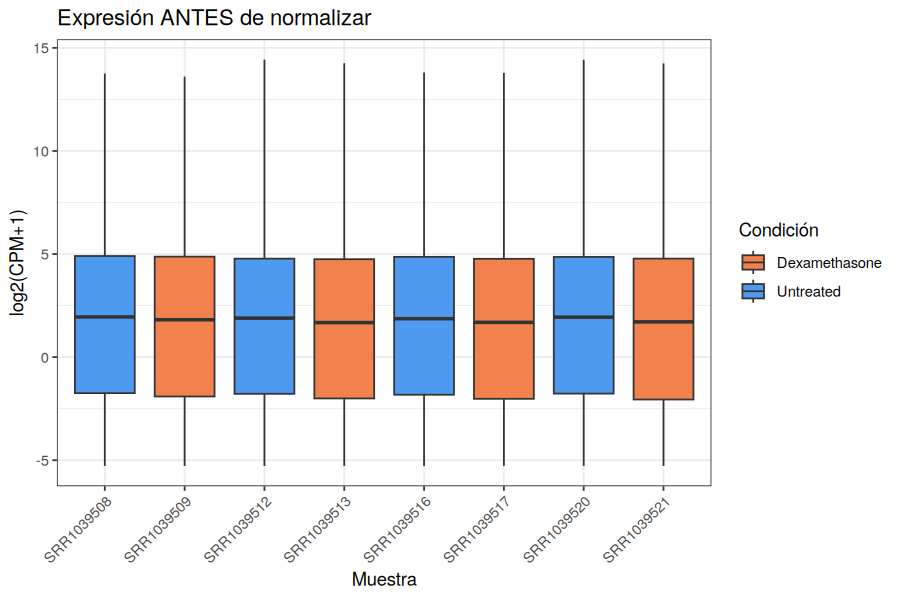
\includegraphics[width=\textwidth]{imagenes/boxplot_raw.png}
            \captionof{figure}{Distribución de expresión cruda (log2 CPM+1) para las 8 muestras. Las medianas y rangos intercuartílicos son homogéneos entre muestras, indicando librerías de tamaño similar.}
        \end{minipage}
        \hspace{0.5cm}
        \begin{minipage}{0.45\textwidth}
            \centering
            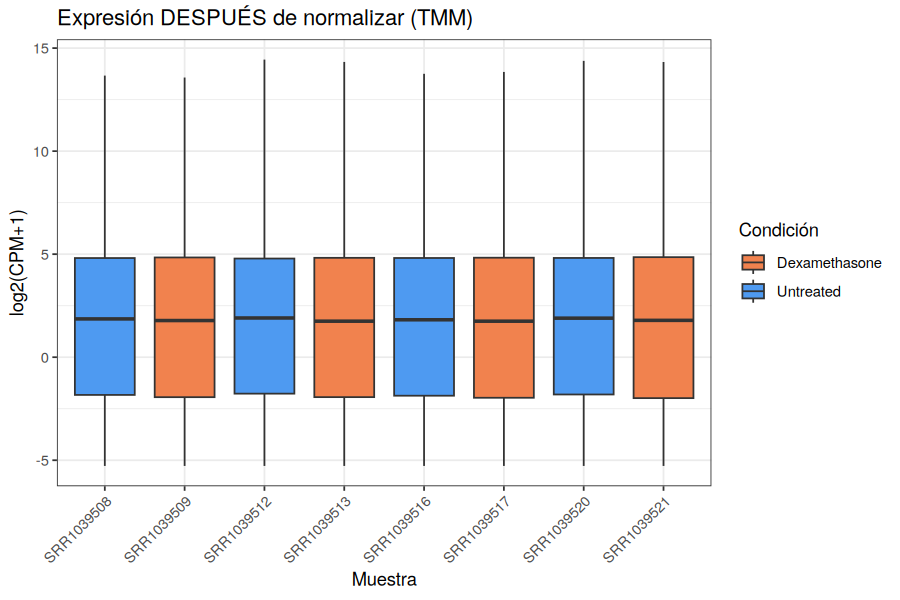
\includegraphics[width=\textwidth]{imagenes/boxplot_normalized.png}
            \captionof{figure}{Distribución de expresión tras normalización TMM. Los leves ajustes confirman que las librerías estaban bien equilibradas y que la normalización fue efectiva.}
        \end{minipage}
        \end{figure}

    \item \textbf{PCA (Análisis de Componentes Principales):} El PCA no supervisado resume la variabilidad global del transcriptoma usando los 500 genes de mayor varianza. PC1 (29.9\% de varianza explicada) separa claramente las muestras \textit{Untreated} (azul) de las \textit{Dexamethasone} (naranja), confirmando que el tratamiento farmacológico es el principal factor de variación en el transcriptoma. PC2 (28.1\%) refleja la variabilidad entre donantes, coherente con el diseño pareado 4×2 del experimento.

    Se observan dos muestras con comportamiento atípico: \texttt{SRR1039516} (donante N080611, Untreated) y \texttt{SRR1039517} (donante N08611, Dexamethasone). Ambas corresponden al mismo donante, pero sus identificadores presentan una discrepancia tipográfica en los metadatos originales de GEO (\texttt{N080611} vs \texttt{N08611}). Esta inconsistencia, junto con posibles diferencias técnicas en la calidad de secuenciación de ese donante, explicaría su separación del resto. El patrón general de separación por condición se mantiene para las 6 muestras restantes, por lo que este hallazgo no compromete la validez del análisis.

        \begin{figure}[H]
            \centering
            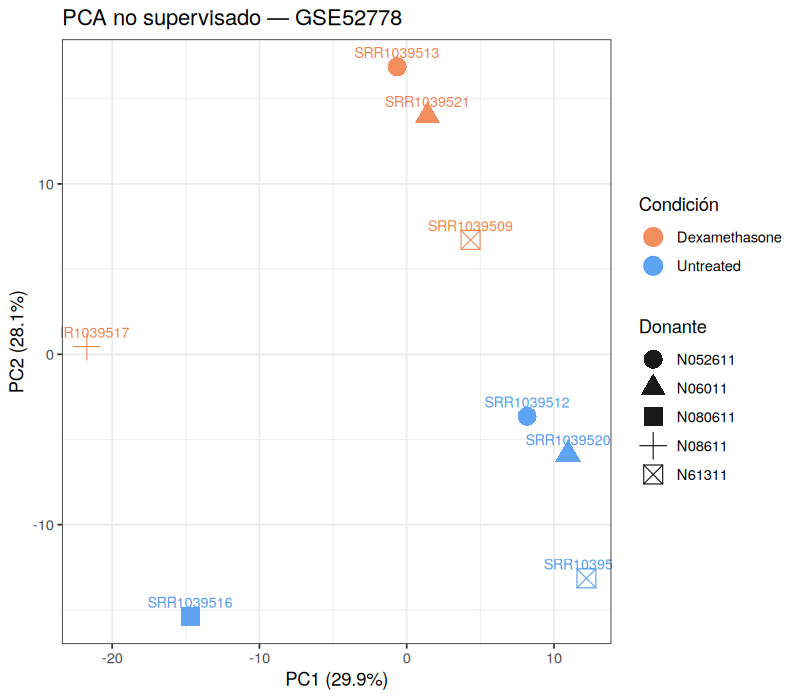
\includegraphics[width=0.5\textwidth]{imagenes/pca_plot.png}
            \caption{PCA no supervisado de las 8 muestras (500 genes de mayor varianza). PC1 separa por condición experimental (Dexamethasone vs Untreated) y PC2 refleja el efecto del donante. Las muestras SRR1039516 y SRR1039517 presentan comportamiento atípico, posiblemente relacionado con una discrepancia en los metadatos del donante.}
        \end{figure}
\end{itemize}

% =============================================================================
% 8. INSTRUCCIONES DE REPRODUCCIÓN
% =============================================================================
\section{Instrucciones de Reproducción}
\label{sec:reproduccion}

\subsection{Requisitos Previos}

Antes de ejecutar el pipeline, es necesario preparar los datos de secuenciación, el genoma de referencia y las imágenes de contenedor:

\begin{verbatim}
# 1. Datos FASTQ (requiere sra-toolkit y pigz)
chmod +x scripts/download_data.sh
./scripts/download_data.sh

# 2. Genoma de referencia (GRCh38 + GTF Ensembl 111)
chmod +x scripts/prepare_genome.sh
./scripts/prepare_genome.sh

# 3. Imagenes de contenedor (solo para HPC con Singularity)
chmod +x scripts/download_images.sh
./scripts/download_images.sh
\end{verbatim}

Se verificará que la estructura de archivos sea la siguiente:
\begin{verbatim}
data/
| SRR1039508/...SRR1039521/
|   | SRR*_1.fastq.gz, SRR*_2.fastq.gz
| genome/
    | GRCh38.fa, GRCh38.gtf
\end{verbatim}

\subsection{Ejecución Local (Docker)}

Para ejecutar el pipeline en un entorno local con Docker:

\begin{verbatim}
nextflow run scripts/main.nf -profile docker
\end{verbatim}

Para reanudar una ejecución interrumpida:
\begin{verbatim}
nextflow run scripts/main.nf -profile docker -resume
\end{verbatim}

\subsection{Ejecución en HPC Picasso (Singularity)}

La ejecución en el clúster Picasso se realiza a través de un script de sumisión para Slurm, \texttt{scripts/script.sh}. Este script solicita los recursos necesarios para el controlador de Nextflow y luego lanza el pipeline. Es importante destacar que, aunque el controlador de Nextflow se ejecuta en el nodo asignado, cada proceso individual del pipeline (FastQC, Trimmomatic, STAR\_ALIGN, etc.) se envía como un trabajo de Slurm independiente gracias al executor configurado en el perfil \texttt{picasso} de \texttt{nextflow.config}.

El comando para lanzar el pipeline es:

\begin{verbatim}
sbatch scripts/script.sh
\end{verbatim}

Para reanudar una ejecución interrumpida, el script \texttt{script.sh} ya incluye la flag \texttt{-resume} en el comando de Nextflow, por lo que re-lanzarlo con \texttt{sbatch} reanudará el flujo desde donde se detuvo.

\subsubsection{Contenido del script de lanzamiento (\texttt{script.sh})}

A continuación, se detalla el contenido del script \texttt{scripts/script.sh}, que encapsula toda la configuración necesaria para el entorno HPC:

\begin{verbatim}
#!/bin/bash
###############################################################################
# script.sh — Lanzador SBATCH para el pipeline RNA-seq en Picasso (SCBI-UMA)
#
# Uso:
#   sbatch scripts/script.sh
###############################################################################

#SBATCH --job-name=rnaseq_nf
#SBATCH --nodes=1
#SBATCH --ntasks=1
#SBATCH --cpus-per-task=12
#SBATCH --mem=64G
#SBATCH --time=48:00:00
#SBATCH --output=logs/nf_%j.out
#SBATCH --error=logs/nf_%j.err
#SBATCH --partition=general

set -euo pipefail

# 1. Cargar módulos
module load singularity/3.7.2
module load nextflow/25.10.4

# 2. Verificación de entorno
command -v nextflow >/dev/null 2>&1 || { echo "ERROR: nextflow"; exit 1; }
command -v singularity >/dev/null 2>&1 || { echo "ERROR: singularity"; exit 1; }

# 3. Configurar directorio de trabajo (FSCRATCH para I/O rápido)
if [ -z "$FSCRATCH" ]; then
    export FSCRATCH="$HOME"
fi

# 4. Caché de imágenes Singularity (.sif)
# IMPORTANTE: Las imágenes deben descargarse primero en el login node
#   con bash scripts/download_images.sh
export NXF_OFFLINE=true
export NXF_SINGULARITY_CACHEDIR="$HOME/UEM/nextflow_rnaseq/.singularity_cache"
export SINGULARITY_CACHEDIR="$HOME/UEM/nextflow_rnaseq/.singularity_cache"
mkdir -p "$NXF_SINGULARITY_CACHEDIR"

# 5. Directorio de trabajo de Nextflow
export NXF_WORK="$FSCRATCH/nextflow_rnaseq_work"
mkdir -p "$NXF_WORK"

# 6. Ejecutar pipeline
echo "=== Iniciando pipeline RNA-seq GSE52778 ==="
nextflow run scripts/main.nf -profile picasso -resume
\end{verbatim}

\subsection{Ejecución del Análisis en R (Workaround)}

Como se ha documentado, debido a los problemas de compatibilidad de las librerías de R dentro del contenedor de Bioconductor, el análisis exploratorio debe ejecutarse manualmente utilizando la instalación nativa de R del clúster:

\begin{verbatim}
module load R/4.3.0  # o la versión disponible en el sistema
Rscript scripts/bin/rnaseq_exploratory.R
\end{verbatim}

Los gráficos resultantes (\textit{boxplots} y PCA) se guardarán en el directorio de salida correspondiente.

\end{document}
